\documentclass[12pt]{article}
\usepackage{fullpage,amsmath,amsfonts,mathpazo,microtype,nicefrac,graphicx}
\usepackage{listings}
\usepackage{mathtools}
\DeclarePairedDelimiter{\ceil}{\lceil}{\rceil}
% Set-up for hypertext references
\usepackage{hyperref,color,textcomp}
\definecolor{webgreen}{rgb}{0,.35,0}
\definecolor{webbrown}{rgb}{.6,0,0}
\definecolor{RoyalBlue}{rgb}{0,0,0.9}
\hypersetup{
   colorlinks=true, linktocpage=true, pdfstartpage=3, pdfstartview=FitV,
   breaklinks=true, pdfpagemode=UseNone, pageanchor=true, pdfpagemode=UseOutlines,
   plainpages=false, bookmarksnumbered, bookmarksopen=true, bookmarksopenlevel=1,
   hypertexnames=true, pdfhighlight=/O,
   urlcolor=webbrown, linkcolor=RoyalBlue, citecolor=webgreen,
   pdfauthor={Andrew Ross},
   pdfsubject={Stat 110},
   pdfkeywords={},
   pdfcreator={pdfLaTeX},
   pdfproducer={LaTeX with hyperref}
}
\setlength\parindent{0pt}
\newcommand*{\ttfamilywithbold}{\fontfamily{lmtt}\selectfont}

\begin{document}

\section*{CS205 Homework 2, Group Problem\\ \small Andrew Ross, Shawn Pan, and Nathaniel Burbank}

\subsection*{Breadth-First Search (BFS)}

We initially represented the edges sparsely as linked lists. However, we ran into issues with how OpenAcc handles the pointers. We ended up  representing the edges as 2 arrays. The edges are sorted by the start point, so we only need to track the end points and the offsets. One array \texttt{edges} contains all the edge endpoints. The second array \texttt{offsets} contains all the offsets into the \texttt{edges} array. For convenience, the \texttt{offsets} array contains 1 more entry than the number of nodes such that the corresponding edges starting from node $i$ lie between indicies \texttt{offsets[i]} and \texttt{offset[i+1]} in the \texttt{edges} array.

\subsection*{All-Pairs Shortest Path (APSP)}

First, we implemented the sequential version of the Floyd-Warshall algorithm:

\begin{lstlisting}[language=C,basicstyle=\ttfamilywithbold\footnotesize]
void floyd_apsp(float* D, int n) {
  for (int k = 0; k < n; k++) {
    for (int i = 0; i < n; i++) {
      for (int j = 0; j < n; j++) {
        float detour = D[i*n + k] + D[k*n + j];
        if (detour < D[i*n + j])
          D[i*n + j] = detour;
      }
    }
  }
}
\end{lstlisting}

However, we encountered difficulties trying to parallelize this due to the fact that the outer loop over \texttt{k} must be executed sequentially. Inserting \texttt{\#pragma}s into the inner loops is possible, but leads to slower performance due to the repeated spin-up and spin-down of threads and unnecessary data movement. We tried to specify that data should be copied once at the beginning of the block and reused in the parallel inner loops, but this did not appear to improve performance.

We did succeed in parallelizing the algorithms based on the tropical semiring, however, mostly because they spend the bulk of their time in matrix multiplication operations that we have already learned to code in parallel. We implemented two distinct versions of the parallel semiring-based APSP with separate indexing schemes. In the first, we stored arrays in row-major order, with partitioning and recombining steps at each recursive iteration:

\begin{lstlisting}[language=C,basicstyle=\ttfamilywithbold\footnotesize]
void tropical_apsp(float* A, int n) {
  if (n > 1) {
    int l = n/2;
    size_t size = l*l*sizeof(float);
    float* temp = (float*)malloc(size);

    // manually partition A into quadrants
    float* A11 = (float*)malloc(size);
    float* A12 = (float*)malloc(size);
    float* A21 = (float*)malloc(size);
    float* A22 = (float*)malloc(size);
    float* quadrants[4] = { A11, A12, A21, A22 };
    for (int i = 0; i < n; i++)
      for (int j = 0; j < n; j++)
        quadrants[2*(i>=l)+(j>=l)][(i%l)*l+(j%l)] = A[i*n + j];

    tropical_apsp(A11, l);
    tropical_gemm(A11, A12, temp, l); memcpy(A12, temp, size);
    tropical_gemm(A21, A11, temp, l); memcpy(A21, temp, size);
    tropical_gemm(A21, A12, temp, l); minplace(A22, temp, l);

    tropical_apsp(A22, l);
    tropical_gemm(A22, A21, temp, l); memcpy(A21, temp, size);
    tropical_gemm(A12, A22, temp, l); memcpy(A12, temp, size);
    tropical_gemm(A12, A21, temp, l); minplace(A11, temp, l);

    for (int i = 0; i < l; i++) {
      for (int j = 0; j < l; j++) {
        A[( i )*n+( j )] = A11[i*l+j];
        A[( i )*n+(j+l)] = A12[i*l+j];
        A[(i+l)*n+( j )] = A21[i*l+j];
        A[(i+l)*n+(j+l)] = A22[i*l+j];
      }
    }

    free(A11);
    free(A12);
    free(A21);
    free(A22);
    free(temp);
  }
}

void tropical_gemm(float* A, float* B, float* C, int n) {
  #pragma acc parallel loop copyin(A[:n*n], B[:n*n]) copyout(C[:n*n])
  for (int i = 0; i < n; i++) {
    #pragma acc loop independent
    for (int j = 0; j < n; j++) {
      float c = inf;
      for (int k = 0; k < n; k++)
        c = fmin(c, A[i*n+k] + B[k*n+j]);
      C[i*n+j] = c;
    }
  }
}
\end{lstlisting}

To reduce the number of copy operations required, we realized that for square matrices whose dimensions $n$ are powers of 4, it is possible to index them in a 1D array not in row-major order but recursively such that quadrants map to quarters. Just to enumerate this briefly, for an $8 \times 8$ matrix, the 1D indexes would be as follows:
$$
\begin{bmatrix}
  0  & 1  & 4  & 5  & \\
  2  & 3  & 6  & 7  & \\
  8  & 9  & 12 & 13 & \\
  10 & 11 & 14 & 15 &
\end{bmatrix}
$$

This allows us to implement a slightly simpler APSP routine:

\begin{lstlisting}[language=C,basicstyle=\ttfamilywithbold\footnotesize]
void tropical_quadtree_apsp(float* A, unsigned int n) {
  if (n > 1) {
    int l = n/2;
    size_t size = l*l*sizeof(float);
    float* temp = (float*)malloc(size);
    float* A11 = A;
    float* A12 = A + n*n/4;
    float* A21 = A + n*n/2;
    float* A22 = A + 3*n*n/4;

    tropical_quadtree_apsp(A11, l);
    tropical_quadtree_gemm(A11, A12, temp, l); memcpy(A12, temp, size);
    tropical_quadtree_gemm(A21, A11, temp, l); memcpy(A21, temp, size);
    tropical_quadtree_gemm(A21, A12, temp, l); minplace(A22, temp, l);

    tropical_quadtree_apsp(A22, l);
    tropical_quadtree_gemm(A22, A21, temp, l); memcpy(A21, temp, size);
    tropical_quadtree_gemm(A12, A22, temp, l); memcpy(A12, temp, size);
    tropical_quadtree_gemm(A12, A21, temp, l); minplace(A11, temp, l);

    free(temp);
  }
}

void tropical_quadtree_gemm(float* A, float* B, float* C, unsigned int n) {
  #pragma acc parallel loop copyin(A[:n*n], B[:n*n]) copyout(C[:n*n])
  for (unsigned int i = 0; i < n; i++) {
    #pragma acc loop independent
    for (unsigned int j = 0; j < n; j++) {
      float c = inf;
      for (unsigned int k = 0; k < n; k++)
        c = fmin(c, A[qx(i,k)] + B[qx(k,j)]);
      C[qx(i,j)] = c;
    }
  }
}
\end{lstlisting}

where the \texttt{qx} function maps 2D indexes to 1D quadtree indexes, which can be done in practice with \href{http://graphics.stanford.edu/~seander/bithacks.html#InterleaveBMN}{interleaving bits}. However, in practice, this performed slightly slower than our normal tropical semiring APSP implementation, perhaps because for the actual matrix multiplications, we sacrifice the sequential access patterns that make parallelization memory-efficient (since logically adjacent matrix elements are no longer physically adjacent). Another possible reason is the additional computational cost required to translate 1D indexes into quadtree form. Performance results for both versions of the tropical algorithm as compared to the sequential Floyd-Warshall implementation are shown below, benchmarked against RMAT graphs of varying scale factor (edge factor did not appear to have a significant effect on performance):

\begin{center}
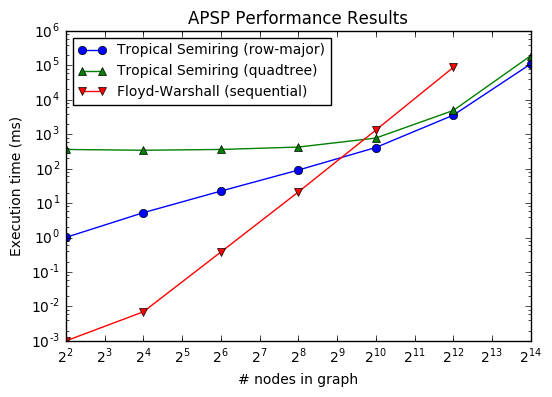
\includegraphics[width=0.67\textwidth]{apsp-results.png}
\end{center}

Note that the sequential Floyd-Warshall algorithm is initially faster because there is no need to copy any data to the GPU, but for large problem sizes, the parallel implementations are over an order of magnitude faster.

We tested our algorithms to ensure they agreed with each other and with the example from the lecture notes. \href{https://github.com/span314/cs205group/blob/master/unit_tests.c}{Unit tests} and the \href{https://github.com/span314/cs205group/blob/master/APSP.c}{APSP code} are available online.

\end{document}

